\section{Quetzal 1 y 2}

  % #figure(
  %   image("./images/Quetzal-2.png"),
  %   caption: [Prototipo conceptual de Quetzal-2. Fuente: Universidad del Valle de Guatemala.]
  % ) <prototype_quetzal2>
\begin{figure}[htbp]
  \centering
  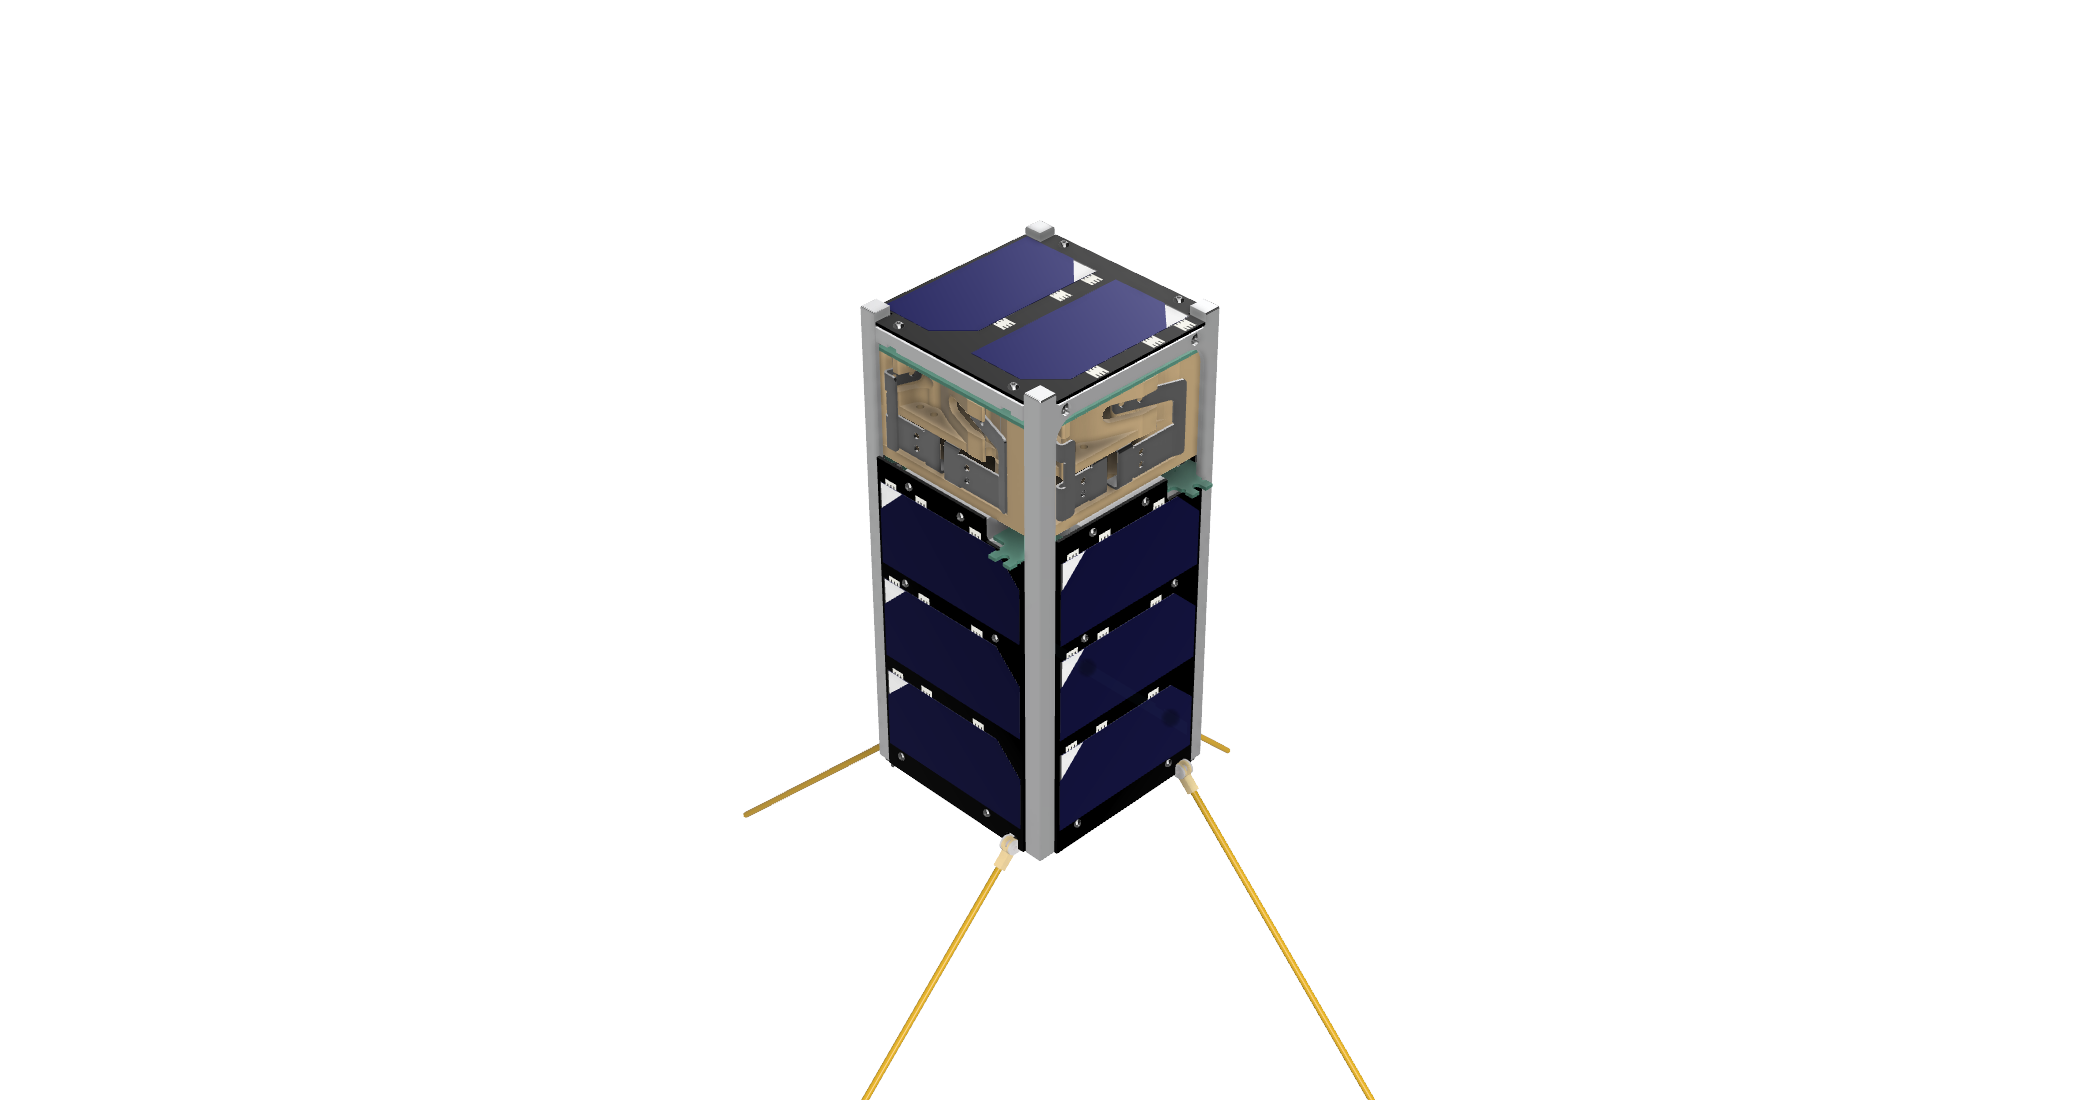
\includegraphics[width=\linewidth]{./images/Quetzal-2.png}
  \caption{Prototipo conceptual de Quetzal-2. Fuente: Universidad del Valle de Guatemala.}
  \label{fig:prototype_quetzal2}
\end{figure}

El Quetzal-2 (\ref{fig:prototype_quetzal2}) es el segundo proyecto aeroespacial de la Universidad del Valle de Guatemala, el cual es desarrollado por estudiantes y personal académico de la institución \cite{quetzal_2}.

  Su predecesor, el Quetzal-1 (\ref{fig:cubesat_quetzal1}), fue el primer satélite guatemalteco, cuya misión buscaba probar un sensor multiespectral para adquirir información remota para conservar recursos naturales de forma independiente \cite{quetzal_1}. El trabajo realizado para Quetzal-1 representa las bases para el nuevo y mejorado Quetzal-2, el cual busca poner a prueba una computadora a bordo (OBC por sus siglas en inglés) diseñada localmente, capaz de ejecutar un modelo de inteligencia artificial para identificar nubes en imágenes satelitales. Así como validará un subsistema para desorbitación responsable y permitirá transmitir datos satelitales en tiempo real a centros educativos del país \cite{quetzal_2}.

  % #figure(
  %   image("./images/Quetzal-1.jpg", width: 40%),
  %   caption: [_CubeSat_ Quetzal 1. Fuente: Universidad del Valle de Guatemala.]
  % ) <cubesat_quetzal1>
\begin{figure}[htbp]
  \centering
  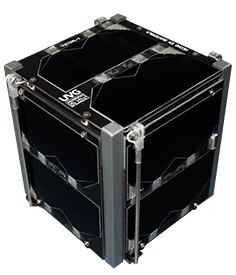
\includegraphics[width=0.4\linewidth]{./images/Quetzal-1.jpg}
	\caption{\textit{CubeSat} Quetzal 1. Fuente: Universidad del Valle de Guatemala.}
  \label{fig:cubesat_quetzal1}
\end{figure}

  Debido a la complejidad de la misión, Quetzal-2 es un CubeSat 2U, el doble de tamaño que su predecesor \cite{quetzal_2}. CubeSat es un estándar que inició en 1999, desarrollado por el profesor Jordi Puig-Sauri y Bob Twiggs. La intención de este estándar es reducir costos y tiempos de desarrollo, al mismo tiempo que incrementa la accesibilidad al espacio. Todos los satélites CubeSat adoptan un tamaño y peso medido en unidades ('U'), la medida que define el estándar. Un CubeSat de 1U (como el Quetzal-1 \cite{quetzal_1}) es un centímetro de 10cm de lado con una masa de hasta 2kg \cite{cubesat_2022}.

\section{Computadora a Bordo (OBC)}

  Esta clase de misiones espaciales se componen de varios subsistemas comunicándose entre sí para llevar a cabo el objetivo de la misión, de esta realidad surge la necesidad de una OBC, la cual se encarga de manejar y dirigir de forma autónoma estas comunicaciones, así como la interacción con la estación de control terrena (GCS por sus siglas en inglés) \cite{lwabanji_wilkinson_biermann_bellville_2013}.

  Según Gildeh \cite{gildeh_2003}, un CubSat típico se compone de varios subsistemas, como mínimo:
\begin{itemize}
  \item Sistema de poder (EPS por sus siglas en inglés), cargado por paneles solares.
  \item Una carga útil (comúnmente llamada \textit{payload}), el/los objetivo(s) de la misión, generalmente una cámara o similar.
  \item Sistema de control y determinación de altura (ADCS por sus siglas en inglés).
  \item Sistema de comunicación por radiofrecuencia.
  \item Una OBC que permite la comunicación entre todos estos subsistemas.
\end{itemize}

  En el caso de Quetzal-2, la OBC realmente se divide en 2, una principal y una secundaria. La OBC principal, es la misma que se utilizó en Quetzal-1, la Gomspace Nanomind A3200 \cite{ayerdi_2023}, esta computadora fue especialmente diseñada para misiones espaciales, como sensores integrados para control de actitud y protecciones especiales contra radiación \cite{gomspace_2026}.

  La OBC secundaria, la cual es diseñada localmente, está compuesta por una pareja de Portentas H7 Lite, ambas cuentan con dos cores de procesamiento y 8MB de SDRAM \cite{arduino_2026}. La OBC secundaria, al igual que la primaria, necesita gestionar la comunicación entre los distintos subsistemas, por lo que se le considera el cerebro del satélite \cite{lwabanji_wilkinson_biermann_bellville_2013} y según \cite{stras2003design} necesita cumplir con las siguientes tareas:
\begin{itemize}
	\item {Grabar y guardar la telemetría del satélite, incluyendo la data de las \textit{payloads} y su transmisión hacia la GCS.}
  \item {Cifrado y descifrado de los paquetes de datos enviados y recibidos de la GCS.}
  \item {Monitoreo y gestión de subsistemas, incluso reiniciando los que sean necesarios.}
\end{itemize}

  Generalmente, la OBC no se encarga de el manejo de energía, en su lugar un subsistema por aparte (el EPS) se encarga de apagar y reinciar sistemas dentro del satélite. Aunque sí hay casos en donde tal tarea se le atribuye a la OBC \cite{hidayat_2010}. La \ref{fig:obc_components} muestra cómo se organizan los componentes de la OBC de Quetzal-2 así como la forma de comunicación con otros submódulos:

  % #figure(
  %   image("./images/OBC_Diagram.png"),
  %   caption: [Diagrama de componentes de la OBC y sus protocolos de comunicación.]
  % ) <obc_components>
\begin{figure}[htbp]
  \centering
  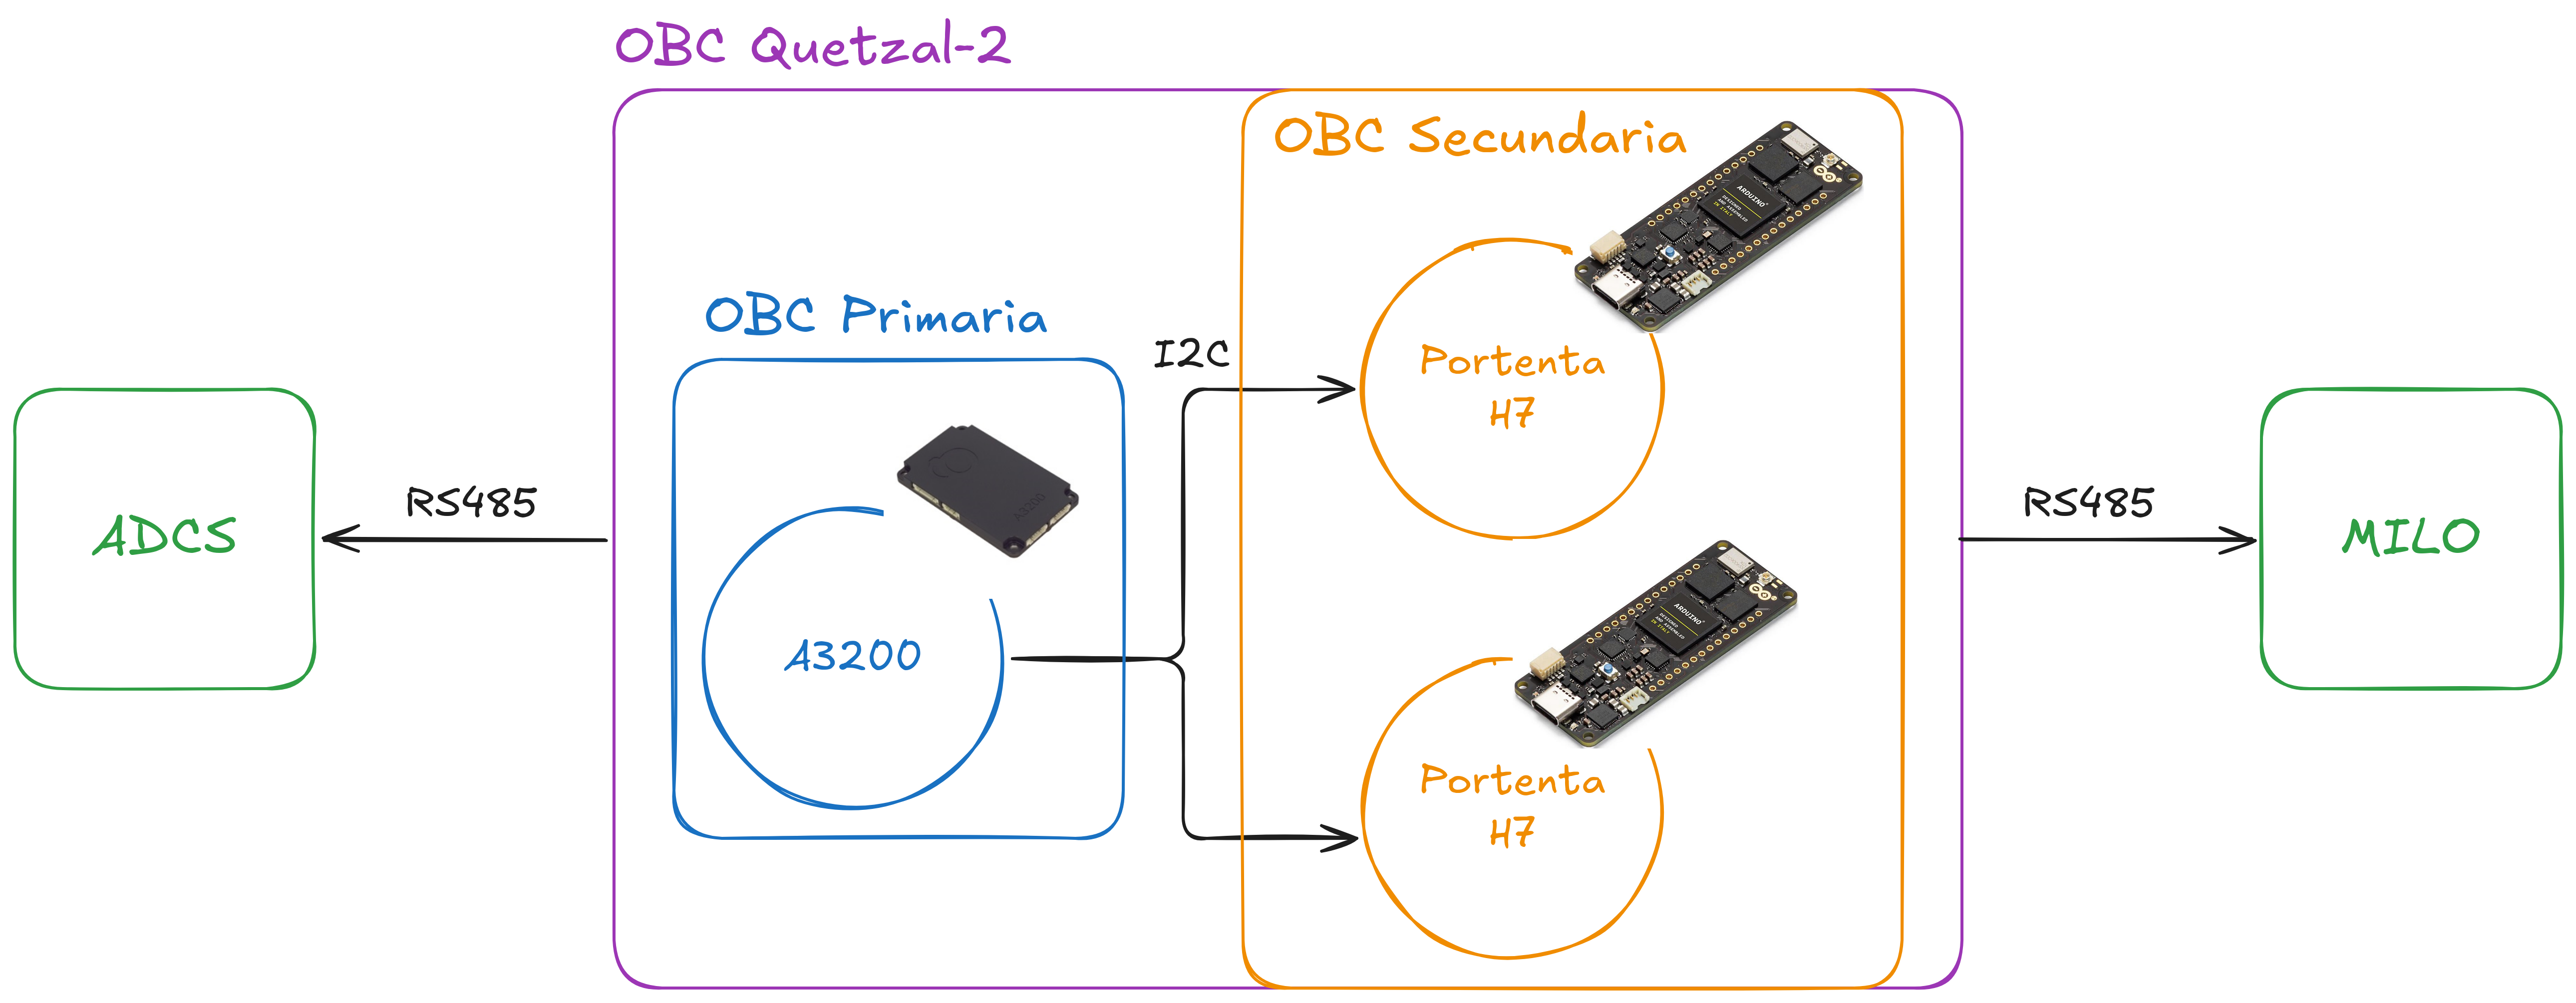
\includegraphics[width=\linewidth]{./images/OBC_Diagram.png}
	\caption{Diagrama de componentes de la OBC y sus protocolos de comunicación.}
  \label{fig:obc_components}
\end{figure}

  \section{Comunicación Serial: I2C y RS485}

  Existen varias interfaces seriales de comunicación que se pueden utilizar para la intercomunicación de microcontroladores, muchas aunque desarrolladas para una aplicación en específico se han vuelto universales, RS485 e I2C caen en esta categoría \cite{hung2020flexible}. Dentro del Quetzal-2 se utilizan estos dos protocolos para la comunicación interna entre sus subsistemas, RS485 es especialmente popular debido a que permite conectar múltiples puntos de control utilizando un bus serial, además de ser un protocolo de comunicación probado en producción por años lo que lo hace una opción segura cuanto menos \cite{sastry2015building}. Mientras que I2C facilita la comunicación entre microcontroladores utilizando un modelo de maestro esclavo, en donde solo el maestro puede iniciar la comunicación \cite{carletti2007comunicacion}.

  Dentro de Quetzal-2, los protocolos se utilizan para los siguientes propósitos:
	\begin{itemize}
		\item {RS485: Comunica la OBC primaria y secundaria con el resto de subsistemas del satélite, es decir: \textit{Payload} MILO, \textit{ADCS}, \textit{EPS}, \textit{Payload} LORA, etc. Se utiliza el protocolo de \textit{hardware} UART para su implementación.}
	\item {I2C: Se utiliza para la comunicación entre la OBC primaria y la OBC secundaria, siendo la OBC primaria la maestra y la OBC secundaria la esclava. Esta decisión es clave para el funcionamiento de la arquitectura de \textit{handover}.}
	\end{itemize}

\subsection{UART}
  El protocolo \textit{Universal Asynchronous Receiver-Transmitter} (UART) es uno de los protocolos de hardware más usados para comunicación entre dispositivos. El protocolo necesita de dos pines: uno para recibir información, llamado comúnmente `RX` y otro para enviar información, llamado `TX`. Ambos se conectan de forma cruzada entre los dispositivos para lograr así la recepción y comunicación de datos en ambos dispositivos \cite{pena2020uart}, como se ve en la \ref{fig:uart_pins}.

  % #figure(
  %   image("./images/UART_Pins.png"),
  %   caption: [Diagrama de conexión de pines entre dos dispositivos que soportan el protocolo de comunicación UART.]
  % ) <uart_pins>
\begin{figure}[htbp]
  \centering
  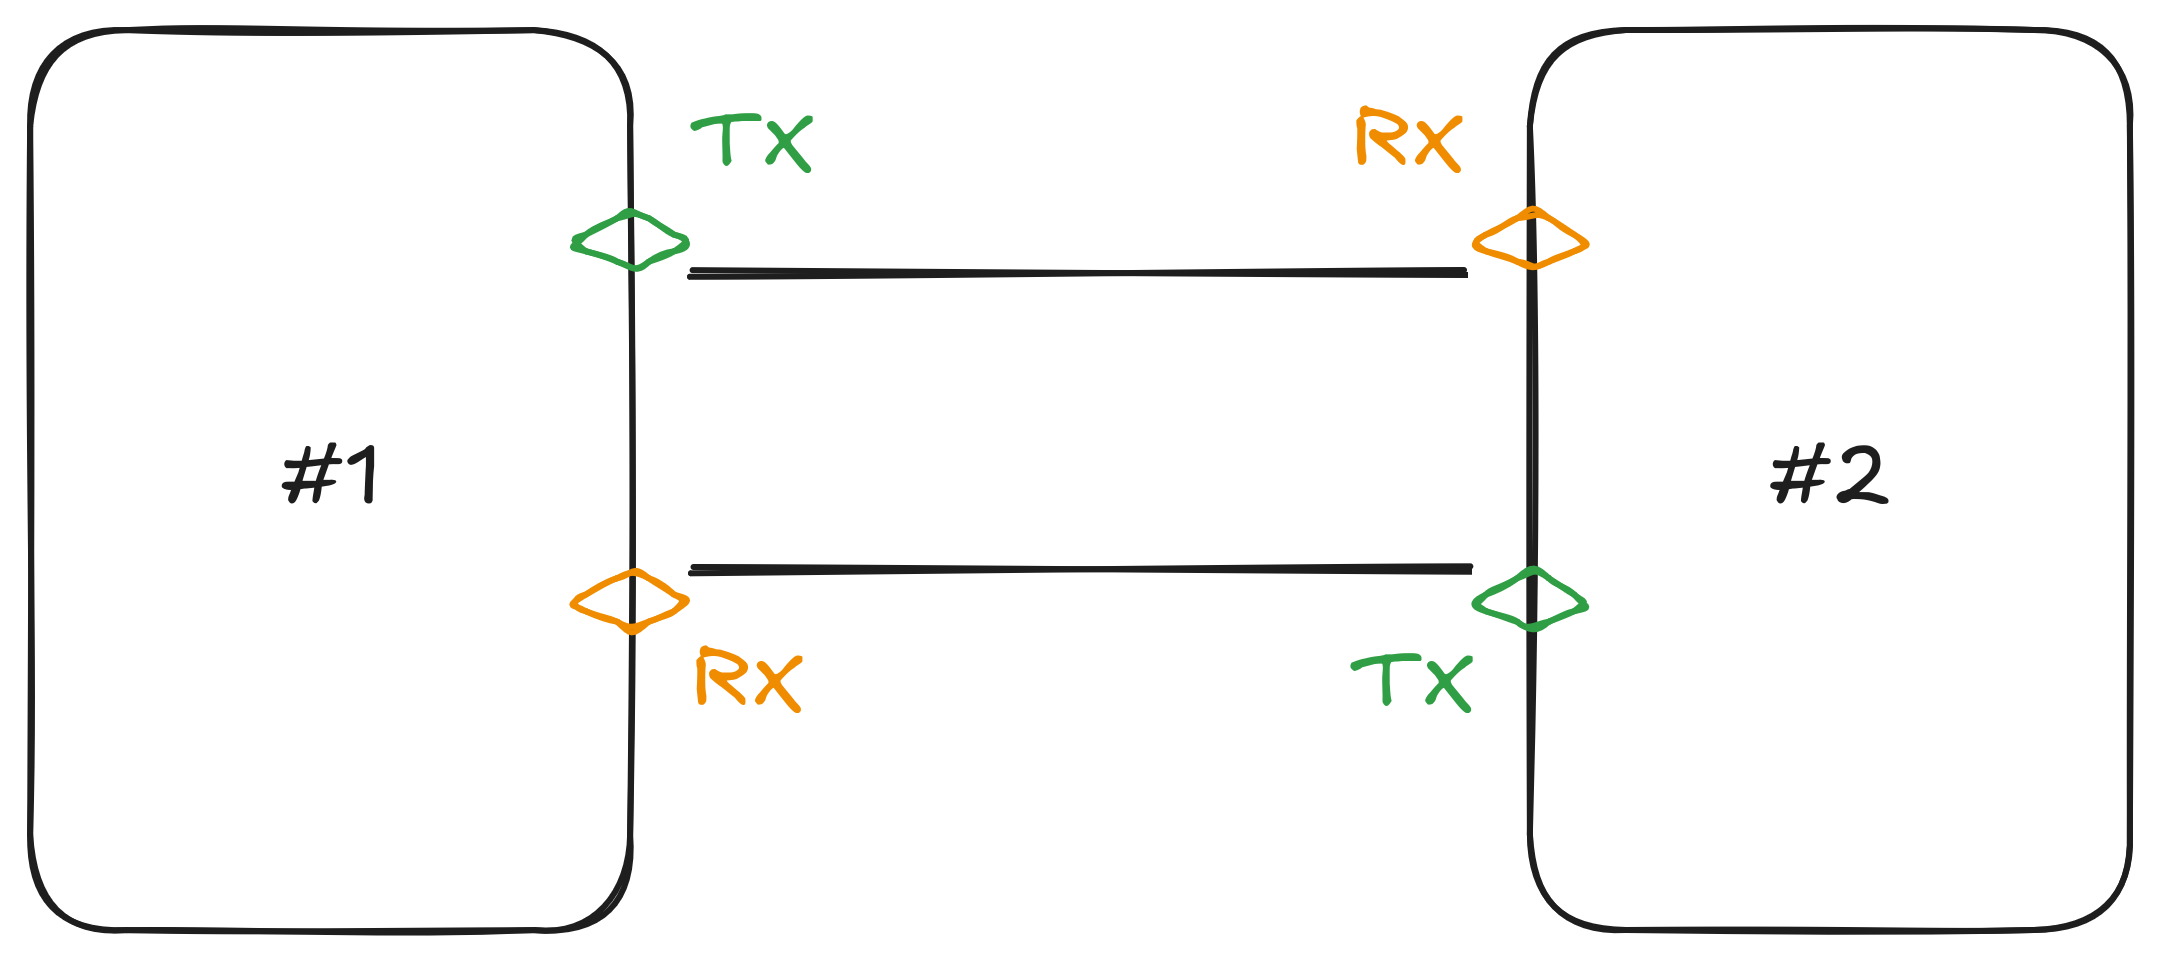
\includegraphics[width=\linewidth]{./images/UART_Pins.png}
	\caption{Diagrama de conexión de pines entre dos dispositivos que soportan el protocolo de comunicación UART.}
  \label{fig:uart_pins}
\end{figure}

  \subsection{RS485}
  El protocolo RS485 se basa en el protocolo RS422, su principal ventaja con respecto a RS422 es que permite la conexión de hasta 32 dispositivos (tanto transmisores como receptores) mientras que RS422 solamente admite 10 receptores y un transmisor. RS485 hereda de RS422 su alta resistencia al ruido, ya que utiliza un voltaje diferencial entre dos cables para transmitir la señal, cuya conexión se ve en la \ref{fig:rs485_pins}. Lo que significa que un byte que se transmite no es un pulso de corriente dentro de un solo cable, sino una diferencia de corriente entre ambas líneas de conexión del protocolo, el \ref{tab:rs485_truth_table} muestra una tabla de verdad con la entrada y cómo se transmite por los cables. Al protocolo solamente le interesa la diferencia entre ambas líneas, por lo que mientras pueda interpretar a una línea como 0 y a otra como 1 seguirá funcionando, lo que lo hace altamente resiliente a ruido \cite{sonnenberg2018serial}.

  % #figure(
  %   image("./images/RS485_Pins.png"),
  %   caption: [Diagrama de conexión de pines entre dos dispositivos que soportan el protocolo de comunicación UART.]
  % ) <rs485_pins>
\begin{figure}[htbp]
  \centering
  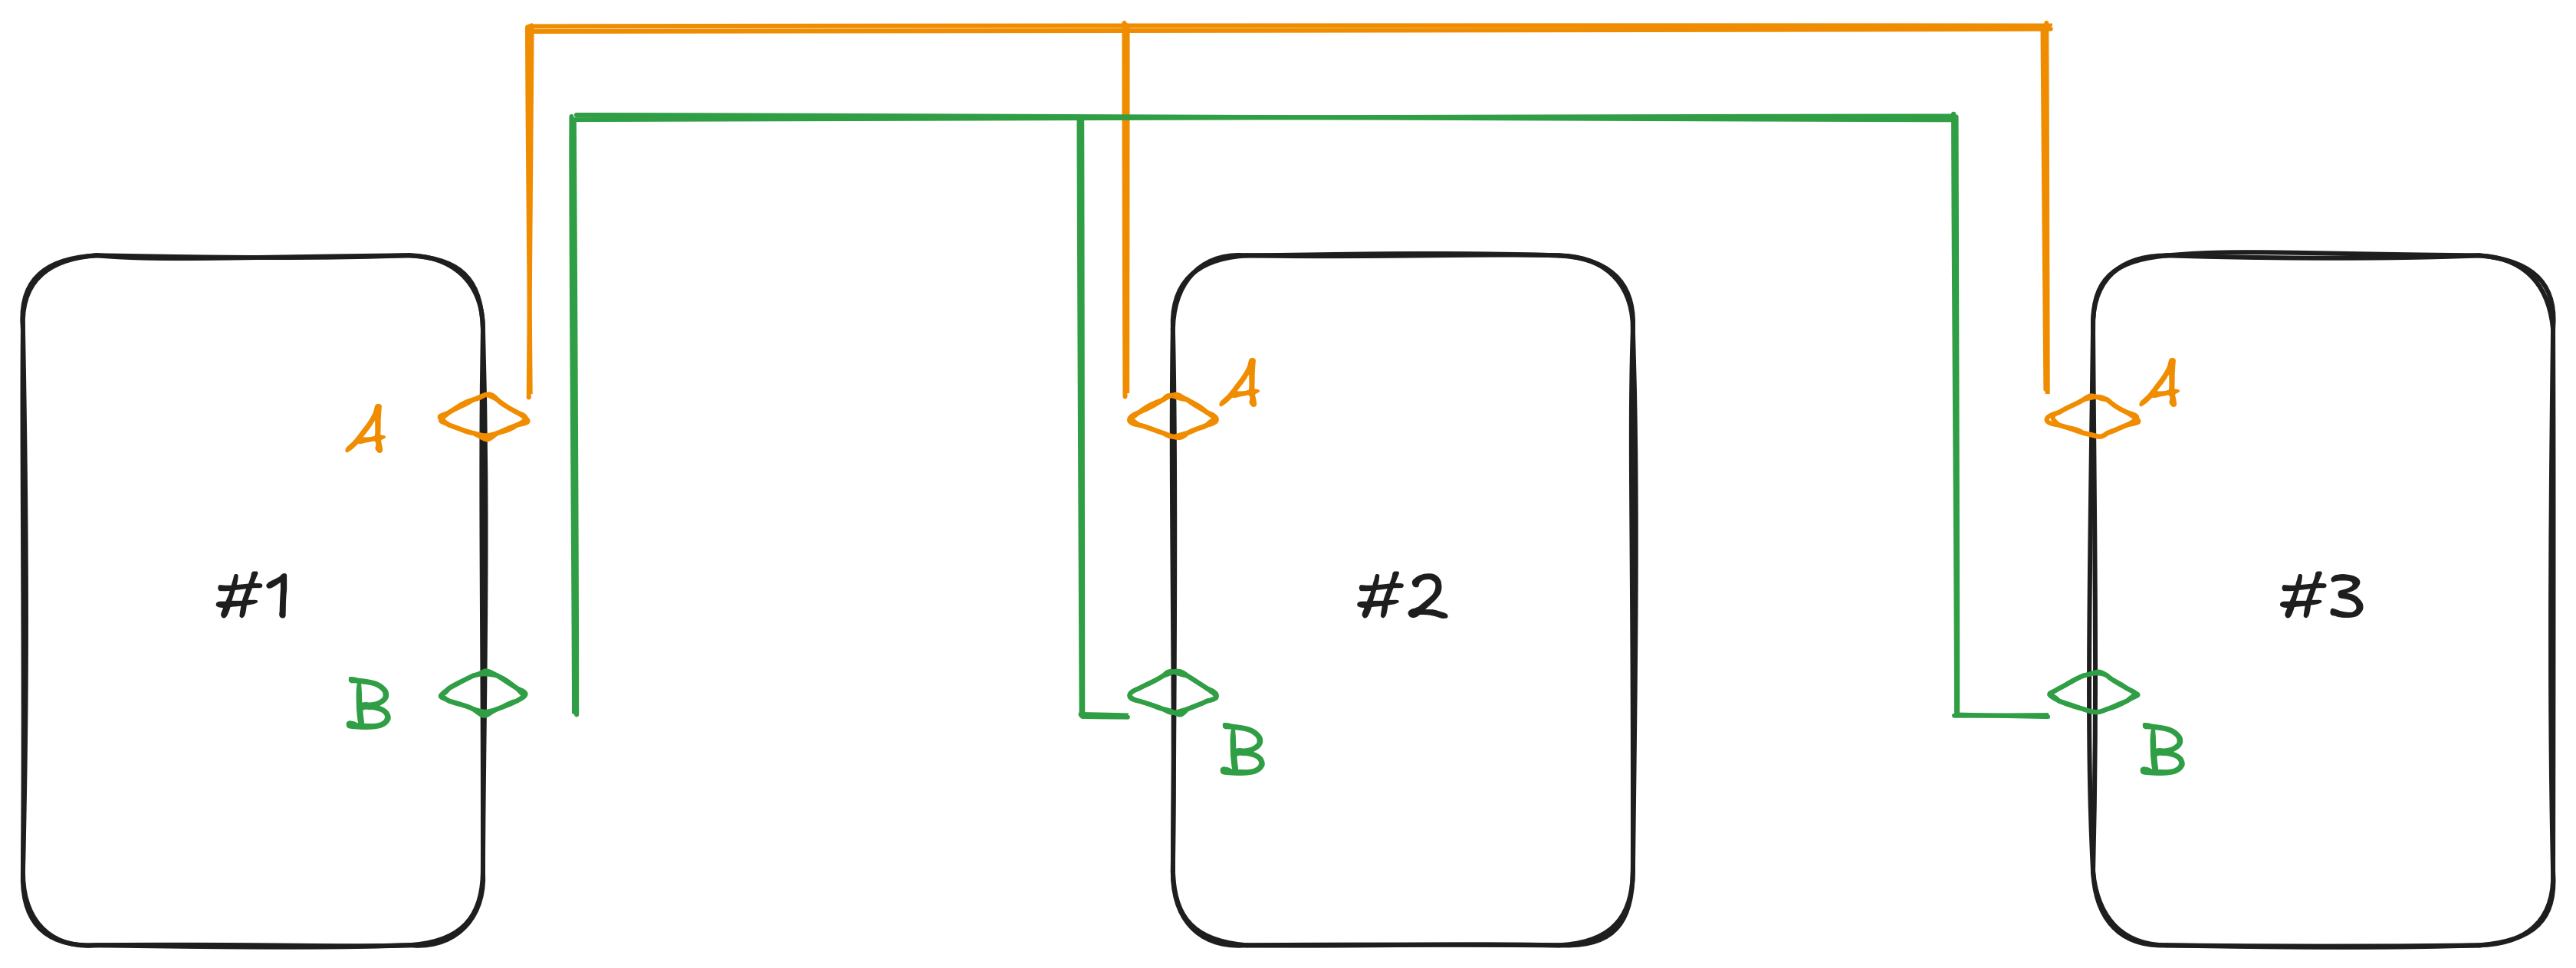
\includegraphics[width=\linewidth]{./images/RS485_Pins.png}
	\caption{Diagrama de conexión de pines entre dos dispositivos que soportan el protocolo de comunicación RS485.}
  \label{fig:rs485_pins}
\end{figure}

  % #figure(
  %   table(
  %     columns: (auto, auto, auto, auto),
  %     align: horizon,
  %     table.header(
  %       [*Entrada*],[*A*],[*B*],[*Salida*],
  %     ),
  %     [0],[1],[0],[0],
  %     [1],[0],[1],[1],
  %   ),
  %   caption: [Tabla de verdad del protocolo RS485.]
  % ) <rs485_truth_table>
  \begin{table}[htbp]
    \centering
    \begin{tabular}{cccc}
		\hline
    \textbf{Entrada} & \textbf{A} & \textbf{B} & \textbf{Salida} \\
    \hline
    0 & 1 & 0 & 0 \\
    1 & 0 & 1 & 1 \\
    \hline
    \end{tabular}
    \caption{Tabla de verdad del protocolo RS485.}
    \label{tab:rs485_truth_table}
  \end{table}

  \subsection{I2C}
  Al igual que RS485, I2C es un protocolo de comunicación serial entre dispositivos, la transmisión de datos es serial y sincrónica, lo que implica el paso de un pulso de reloj para sincronizar la salida y entrada de los datos entre los dispositivos. Requiere de dos líneas de conexión \cite{carletti2007comunicacion}:

	\begin{itemize}
\item {SDA (\textit{Serial Data}): Se utiliza para transmitir los datos entre los dispositivos.}
  \item {SCL (\textit{Serial Clock}): Se utiliza para transmitir los pulsos del reloj. Sincronizando el sistema.}
	\end{itemize}

  Un ejemplo de conexión se puede apreciar en la \ref{fig:i2c_pins}.
  % #figure(
  %   image("./images/I2C_Pins.png"),
  %   caption: [Diagrama de conexión de pines entre dos dispositivos que soportan el protocolo de comunicación I2C.]
  % ) <i2c_pins>
\begin{figure}[htbp]
  \centering
  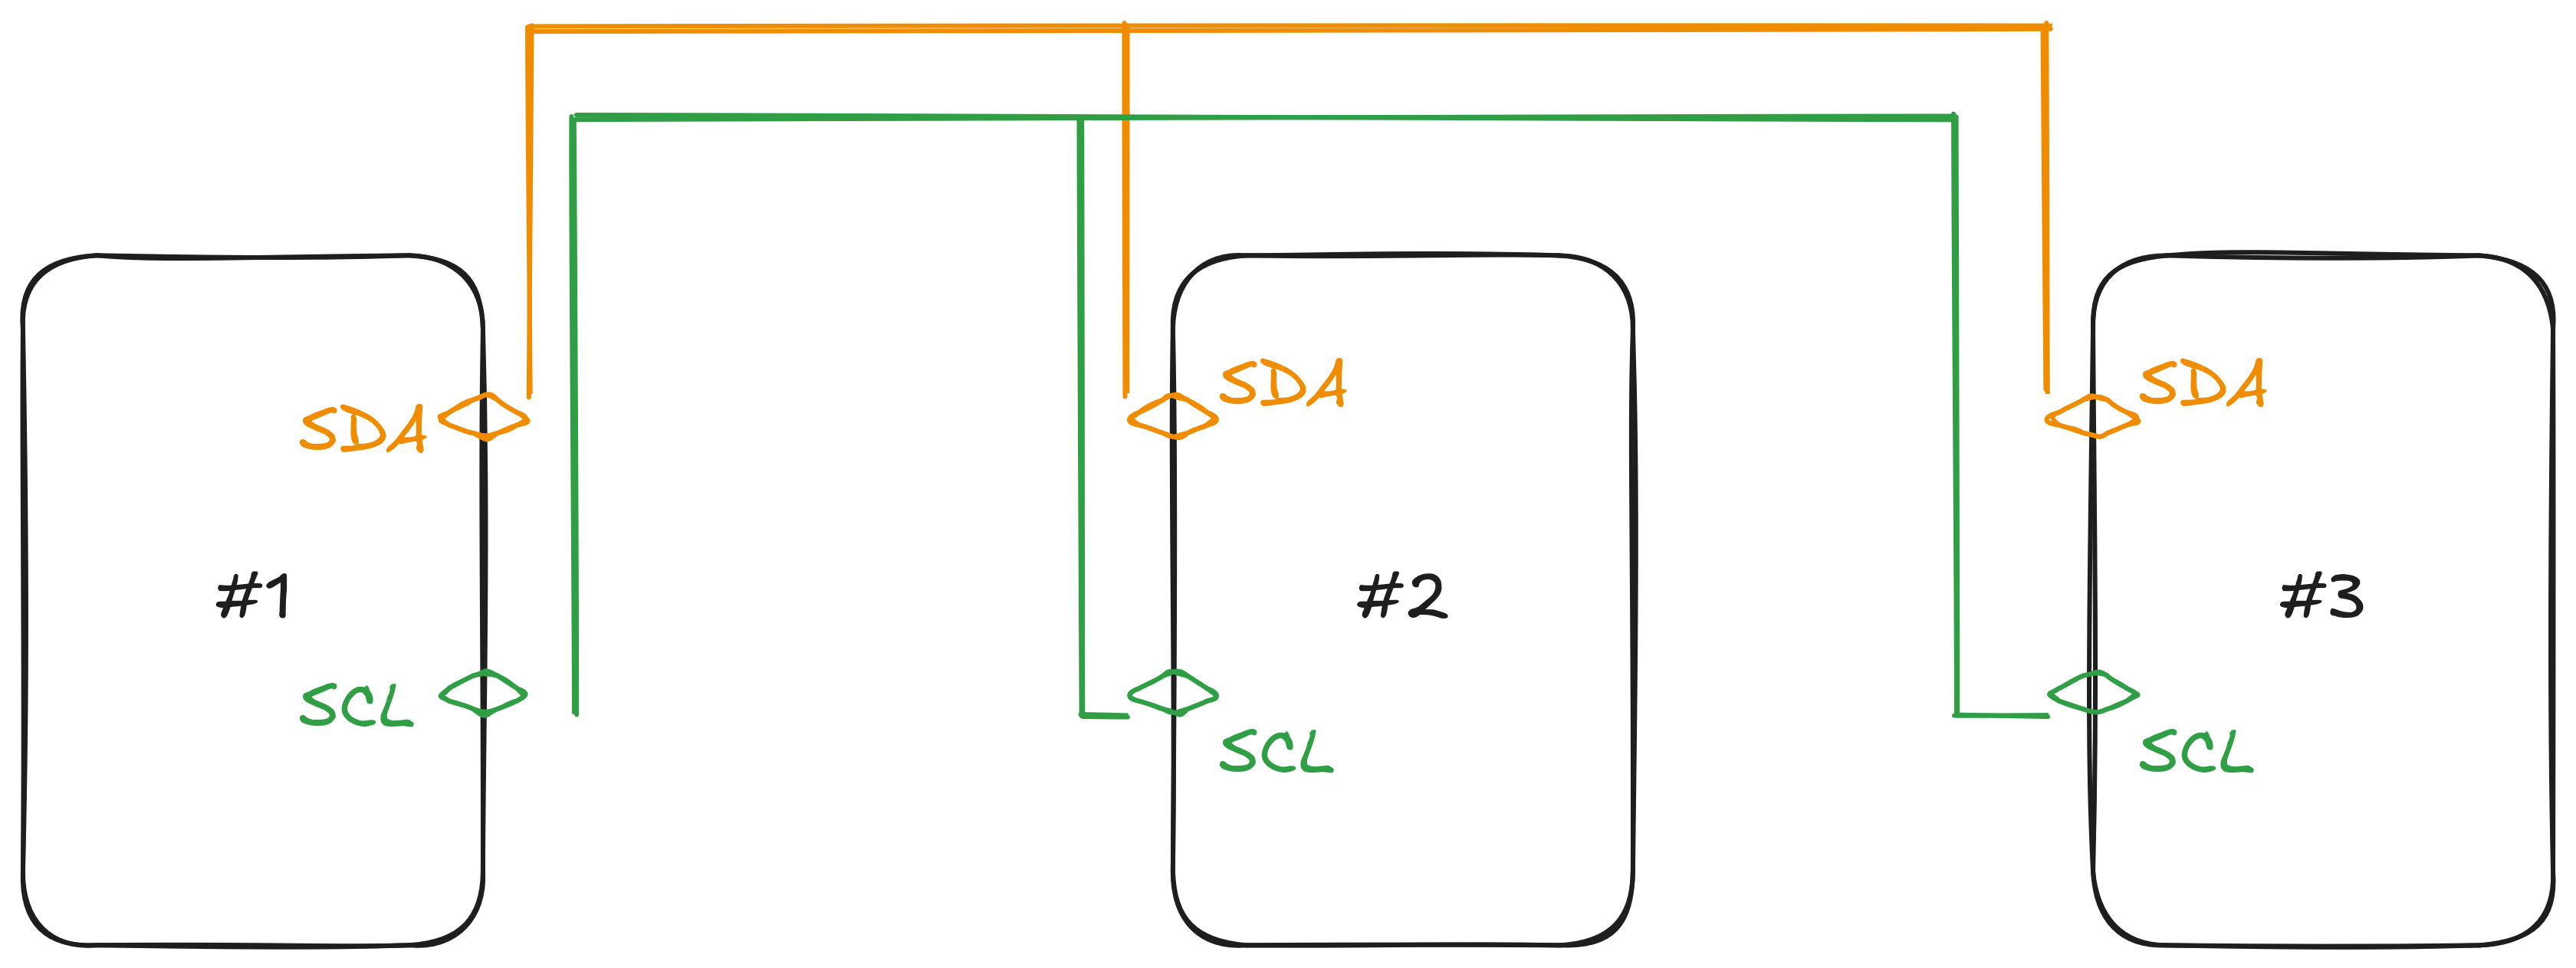
\includegraphics[width=\linewidth]{./images/I2C_Pins.png}
  \caption{Diagrama de conexión de pines entre dos dispositivos que soportan el protocolo de comunicación I2C.}
  \label{fig:i2c_pins}
\end{figure}

  Un detalle importante dentro de este protocolo es el rol que cada dispositivo tiene dentro de la comunicación. Siempre se tiene un dispositivo maestro, encargado de dirigir la comunicación y otros dispositivos esclavos. Estos roles pueden alternar libremente durante \textit{conversaciones} de dispositivos, es posible que para una rutina un microcontrolador sea maestro y para otra sea el esclavo \cite{carletti2007comunicacion}.

  \section{Protocolo de \textit{Handover}}

  El protocolo de \textit{handover} es un sistema interno de la OBC primaria, diseñado localmente, cuyo objetivo principal es trasladar el control del satélite de sí misma a la OBC secundaria de una forma segura y redundante a fallos. Quetzal-2 no es la única misión que ha integrado más de una OBC en su sistema de mando, SHEFEX III, una misión alemana del 2017 también usó dos OBCs para redundancia, sin embargo su estrategia nunca fue ceder control de una OBC a la otra sino tener un backup en caso alguna de la dos fallara \cite{schwarz2014fault}. Otro ejemplo es la arquitectura DHS propuesta en 2023 para misiones académicas como profesionales \cite{soucaille2023high}. Esta arquitectura en específico también se usó en el mismo año para otra misión espacial, la misión HERA, de la misma forma su principal objetivo era redundancia total, pero además buscaba autonomía operacional y alta capacidad de almacenamiento a bordo \cite{Marcos_Valverde_Carretero_2023}.

  Una descripción general del protocolo se puede ver en la \ref{fig:handover_sequence}. En donde se tiene a los 3 actores principales: A3200 representando la computadora principal, Portenta H7, representando la portenta que está activa en ese momento y SAMD, representando a el módulo que se necesita para una tarea, por ejemplo MILO.

  % #figure(
  %   image("./images/OBC_Routines.png"),
  %   caption: [Diagrama de secuencia del protocolo de _handover_ para un caso general.]
  % ) <handover_sequence>
\begin{figure}[htbp]
  \centering
  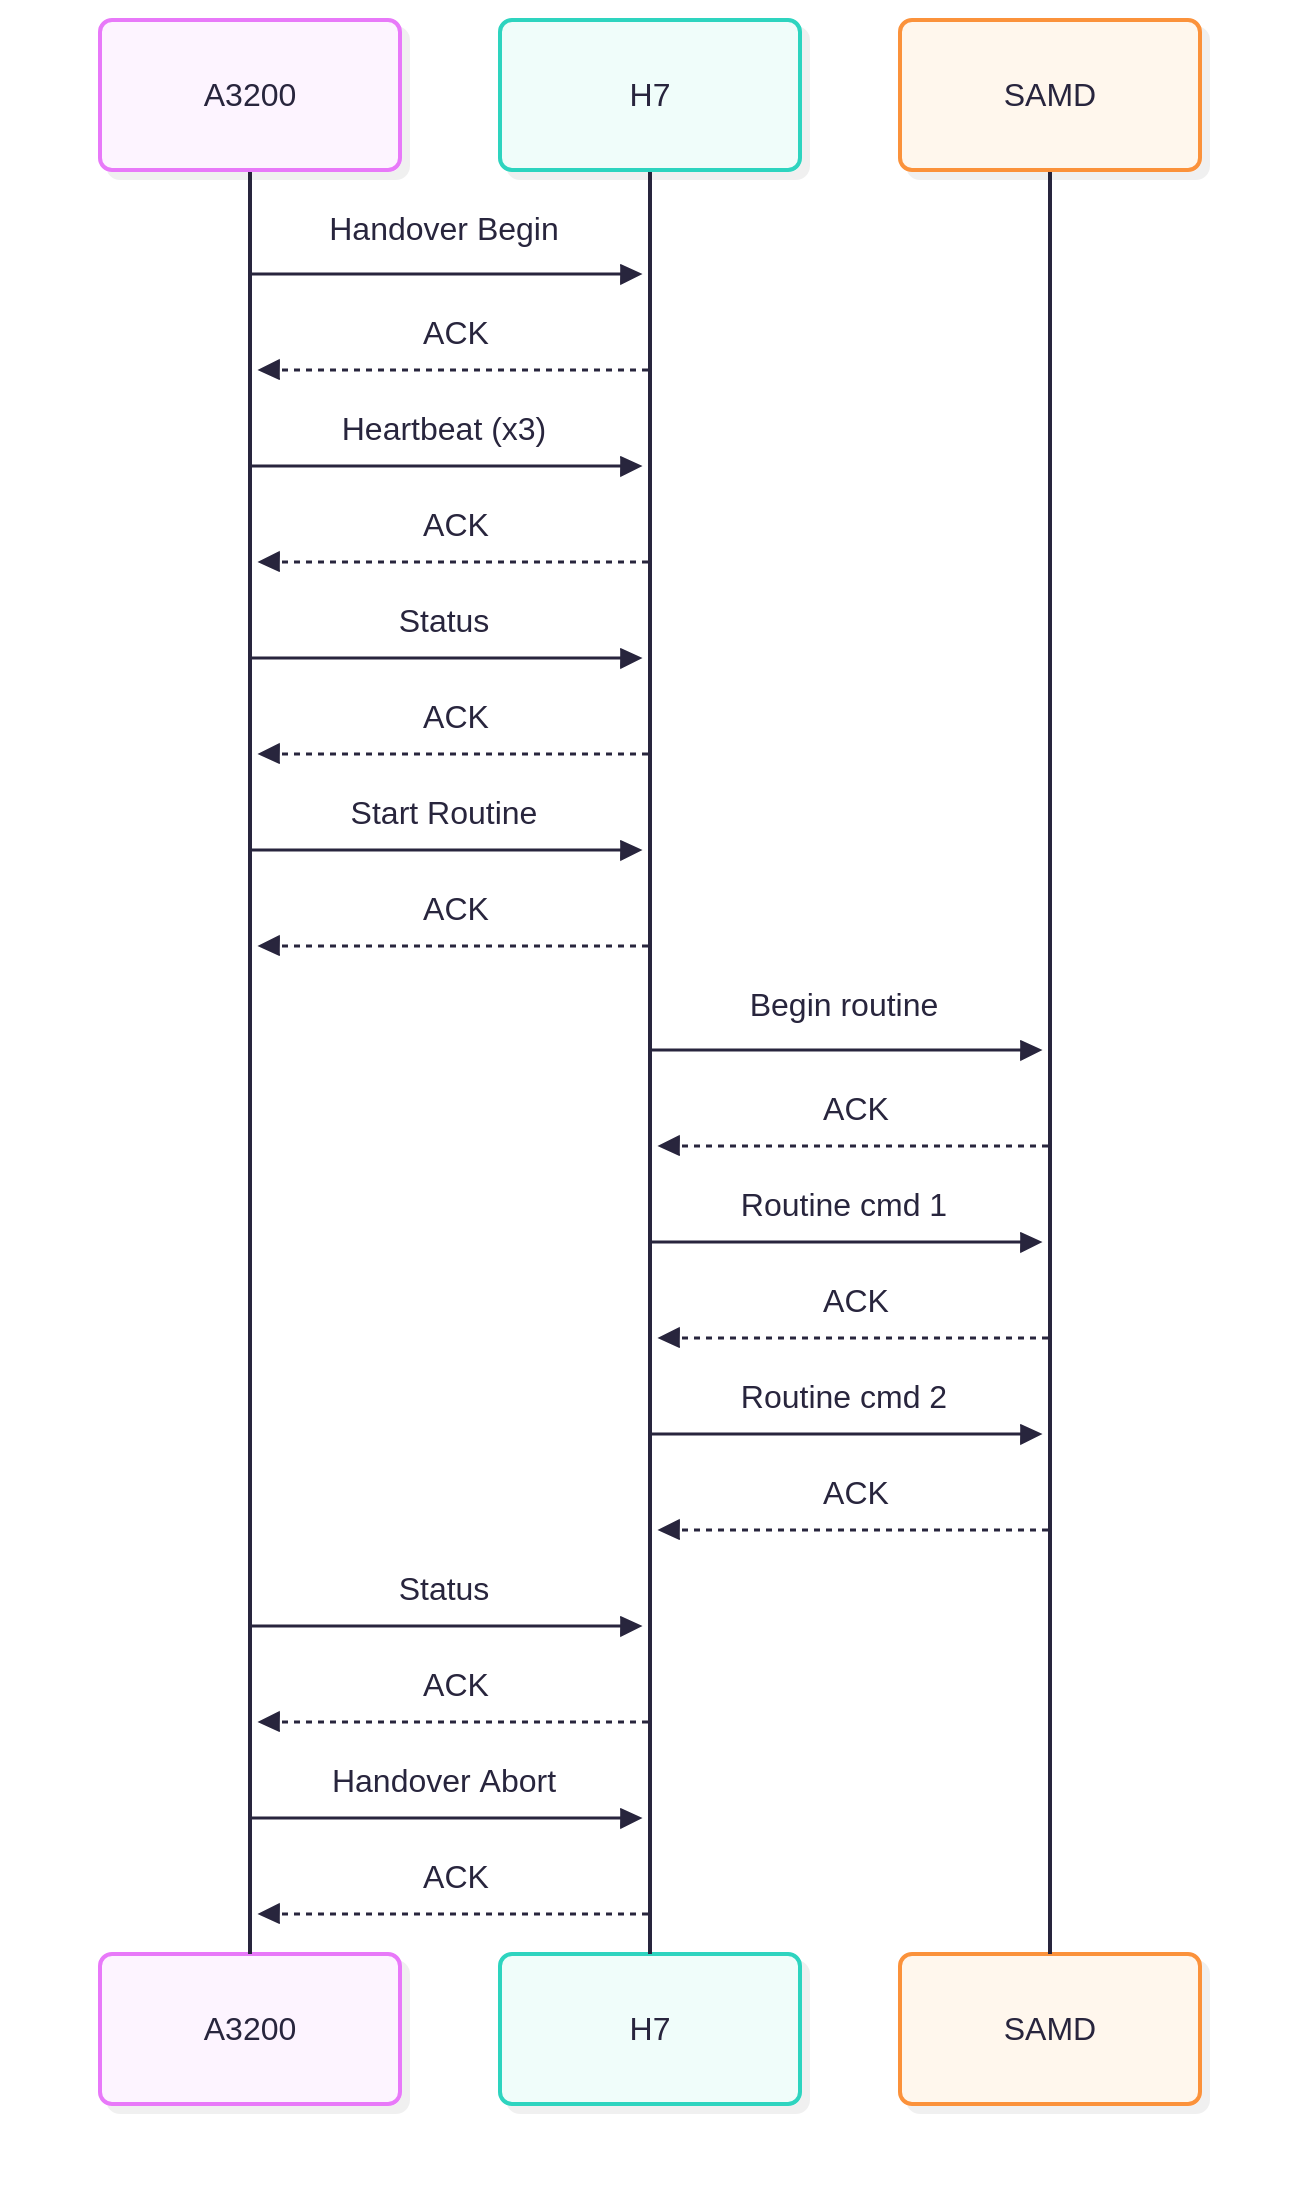
\includegraphics[width=0.8\linewidth]{./images/OBC_Routines.png}
  \caption{Diagrama de secuencia del protocolo de \textit{handover} para un caso general.}
  \label{fig:handover_sequence}
\end{figure}

  En caso de fallos, el comando de \texttt{Handover abort} se enviará de forma automática por la OBC principal, además de que se tendrá un timer que permitirá la toma de control de parte de la OBC primaria en caso la secundaria deje de responder.

  La OBC diseñada localmente es desarrollada en un lenguaje a bajo nivel, particularmente C, debido a que es el lenguaje principal en el que el \textit{driver} a bajo nivel de STM32 es proveído, ofreciendo un mayor control sobre el uso de los recursos, casi tan granular como querramos \cite{stmicroelectronics_2026}. Debido a la complejidad del sistema interno que debe manejar la OBC para gestionar la comunicación entre todos los subsistemas del satélite, se necesita un sistema operativo \cite{lwabanji_wilkinson_biermann_bellville_2013}.

  \section{Sistemas Operativos}
  Existen muchos tipos de sistemas operativos (OS por sus siglas en inglés), según su infraestructura interna podemos tener sistemas operativos monolíticos, por capas, microkernels, módulos o híbridos siendo alguna combinación entre ellos \cite{operating_system_concepts_2018}. Para propósitos del Quetzal-2, resulta de mayor importancia cómo el OS calendariza sus tareas que el cómo se compone internamente el sistema operativo como tal, ya que las misiones espaciales tienden a tener presupuestos muy ajustados tanto de memoria como procesamiento \cite{lwabanji_wilkinson_biermann_bellville_2013}. 

  Los sistemas operativos en tiempo real (RTOS por sus siglas en inglés) fueron creados justamente para los casos en donde se tienen requerimientos de tiempo rígidos \cite{operating_system_concepts_2018} y por esta razón se evaluaron distintas alternativas de implementación de un RTOS. RODOS, un sistema operativo de código abierto desarrollado por Sergio Montenegro, con un énfasis en facilidad de uso, rendimiento y probado en aplicaciones espaciales reales \cite{rodos}; FreeRTOS, otro sistema operativo de código abierto, con una gran comunidad, excelente rendimiento y años de uso en producción \cite{freertos_2010}. Luego de unas pruebas de \textit{porting} de RODOS a STM32H7, la arquitectura de la Portenta H7 Lite, se decidió a utilizar FreeRTOS por su alta compatibilidad con este \textit{hardware}.

  \section{Arquitectura de Software}
  La arquitectura de software busca gestionar la comunicaciónn entre los componentes de software que conforman un sistema \cite{pareja2019arquitectura}. En este caso, sistema se referiría a la OBC diseñada localmente. Al ser una misión espacial, el acceso que tendremos al satélite es muy limitado, no podremos realizar parches de actualización de código por ejemplo. Por lo que tener la mayor garantía que podamos de que el sistema funciona y es resiliente a fallos es la prioridad más alta.

  La \textit{National Aeronautics and Space Administration} (NASA) es famosa por sus 10 reglas para desarrollar código crítico seguro:
	\begin{itemize}
\item{\textbf{No usar recursión, saltos ni \textit{goto statements}}. La justificación de la NASA es debido a que simplificar el flujo de ejecución de nuestro programa generalmente se traduce a mejor claridad del código, así como en una mejora considerable de análisis estático.}
  \item {\textbf{Todos los ciclos deben tener un límite superior fijo}. Sin recursión, y con ciclos que siguen un límite fijo de iteraciones se previene en su totalidad rutinas que se ejecutan de forma indefinida. Esta regla no aplica para rutinas que deben ser forzosamente de terminación indeterminada, como la espera de nuevos comandos de la estación terrena (GCS por sus siglas en inglés).}
  \item {\textbf{No alojar memoria dinámica luego de la inicialización}. La alojación de memoria dinámica impacta negativamente en el rendimiento del sistema, además de que tiene un comportamiento notablemente difícil de predecir con análisis estático. Esta regla fuerza al programador a usar memoria estática alojada al declarar variables en el stack, si se combina con las reglas anteriores el código termina siendo legible y sencillo, lo que es excelente para analizadores estáticos que buscan probar que un programa se comportará como esperamos.}
  \item {\textbf{No más de 60 líneas de código por función}. Funciones extremadamente largas son una señal de código pobremente arquitecturizado.}
  \item {\textbf{Cada función debe tener un promedio de dos \textit{assertions}}. La NASA recomienda utilizar aserciones en el código para probar condiciones de ejecución tanto antes como después de correr una función. Una aserción siempre revisa una condición, en dado caso la condición falle se toma una acción de recuperación que se programó explícitamente para manejar este caso. Las aserciones deben ser libres de efectos secundarios.}
  \item {\textbf{Declara todos los objetos de tipo data en el tamaño mínimo posible de \textit{scope}}. Esta regla simplifica la depuración del código cuando ocurre una falla, puesto que es obvio que una variable que no se encuentra en el scope del código que falla no tiene ninguna relación con el error en sí. Por lo tanto queremos minimizar la cantidad de variables dentro del scope de cada rutina, limitando así, los lugares en donde se puede corromper estado y afectar en la ejecución de nuestro programa.}
  \item {\textbf{Todos los parámetros de retorno deben ser revisados por la función que los llamó}. \textbf{Todas las funciones deben revisar la validez de los parámetros proveídos}. Las interfaces con las que interactuamos los programadores están plagadas de funciones que puede que funcionen como esperamos o no, generalmente tienen una forma de reportar un error. Si una función debe ejecutarse solamente cuando el valor de retorno de otra función es exitoso, entonces es indispensable que este valor de retorno se revise, ese es el corazón de esta regla.}
  \item {\textbf{El uso del preprocesador de C debe estar limitado a inclusión de \textit{header files} y definiciones sencillas}. El preprocesador de C puede fácilmente ofuscar el código y confundir a analizadores estáticos, por lo que la NASA no recomienda su uso más allá de inclusiones sencillas.}
  \item {\textbf{Solamente es permitido un nivel de referencia con punteros}. Según la NASA, los punteros son fácilmente usados de forma incorrecta, incluso por programadores experimentados, pueden hacer que seguir el flujo de control de un programa sea complicado y reestringen las capacidades que tienen los analizadores de código estático.}
  \item {\textbf{Todo el código debe ser compilado desde el primer día de desarrollo con todas las alertas del compilador en la configuración más pedante. El código debe compilar sin advertencias}. Según la NASA, no hay ninguna excusa por la que una \textit{warning} debería ser ignorada, incluyendo los falsos positivos. El código debe ser reescrito para facilitar su análisis estático y no confundir a la herramienta \cite{holzmann_2006}.}
	\end{itemize}

	\subsection{Fiabilidad en \textit{Software}} \label{sec:reliability}
  El espacio no es el único sector dentro del mundo del \textit{software} que necesita una resiliencia extraordinaria. Las bases de datos, son piezas de \textit{software} que deben funcionar incluso si el disco se corrompe, como es el caso de TigerBeetle \cite{greef_2026}. U otra base de datos venerada por su resiliencia a lo largo de los años, SQLite, con más de 1 billón de instancias en uso actualmente \cite{software_should_work_2026}.

  Aunque hechas para casos de uso muy distintos, ambas llegaron a la misma conclusión, la forma de garantizar resiliencia a fallos, incluso en ambientes hostiles, es utilizar el poder de la misma computadora para revisar tu código. No hablan de IA, sino de \textit{fuzz testing}, \textit{unit testing} y otra gran variedad de \textit{xxx testing}. No basta solo el análisis estático, hay que poder garantizar de forma automatizada que la solución funciona y es resiliente a fallos, no porque el \textit{linter} no encuentre errores, sino porque años de simulación que ocurren en horas o días en tiempo real lo respaldan \cite{software_should_work_2026} \cite{greef_2026}.

  \subsubsection{Fuzzing}

  Richard Hipp, uno de los creadores de SQLite, cuenta en su experiencia como desarrollador de este software que al alcanzar 100\% \textit{branch coverage}, dejó de recibir reportes de bugs de sus usuarios por varios años \cite{software_should_work_2026}. Para entender esta métrica es importante entender primero qué es una "rama". En programación se asume que todas las instrucciones ejecutan una luego de la otra, sin embargo esto no siempre es cierto, es común en aplicaciones que ciertas instrucciones sean ejecutadas solamente cuando ciertas condiciones se cumplen. Esto genera bloques de instrucciones por los que el procesador puede o no pasar, todo el conjunto de estos bloques generan un árbol de posibles ejecuciones del programa en donde, según qué condiciones se cumplan, el procesador ejecutará una rama u otra \cite{elmasry2013branchless}. La \ref{fig:branch_simple} demuestra cómo se vería este árbol de ejecución para un programa sencillo.

  % #figure(
  %   image("./images/Ramas_Simple.png", width: 60%),
  %   caption: [Árbol de ejecución de un programa simple. Nótese como cada función genera su propio bloque y algunas ramas tienen condiciones que deben cumplirse para ser ejecutadas.]
  % ) <branch_simple>
\begin{figure}[htbp]
  \centering
  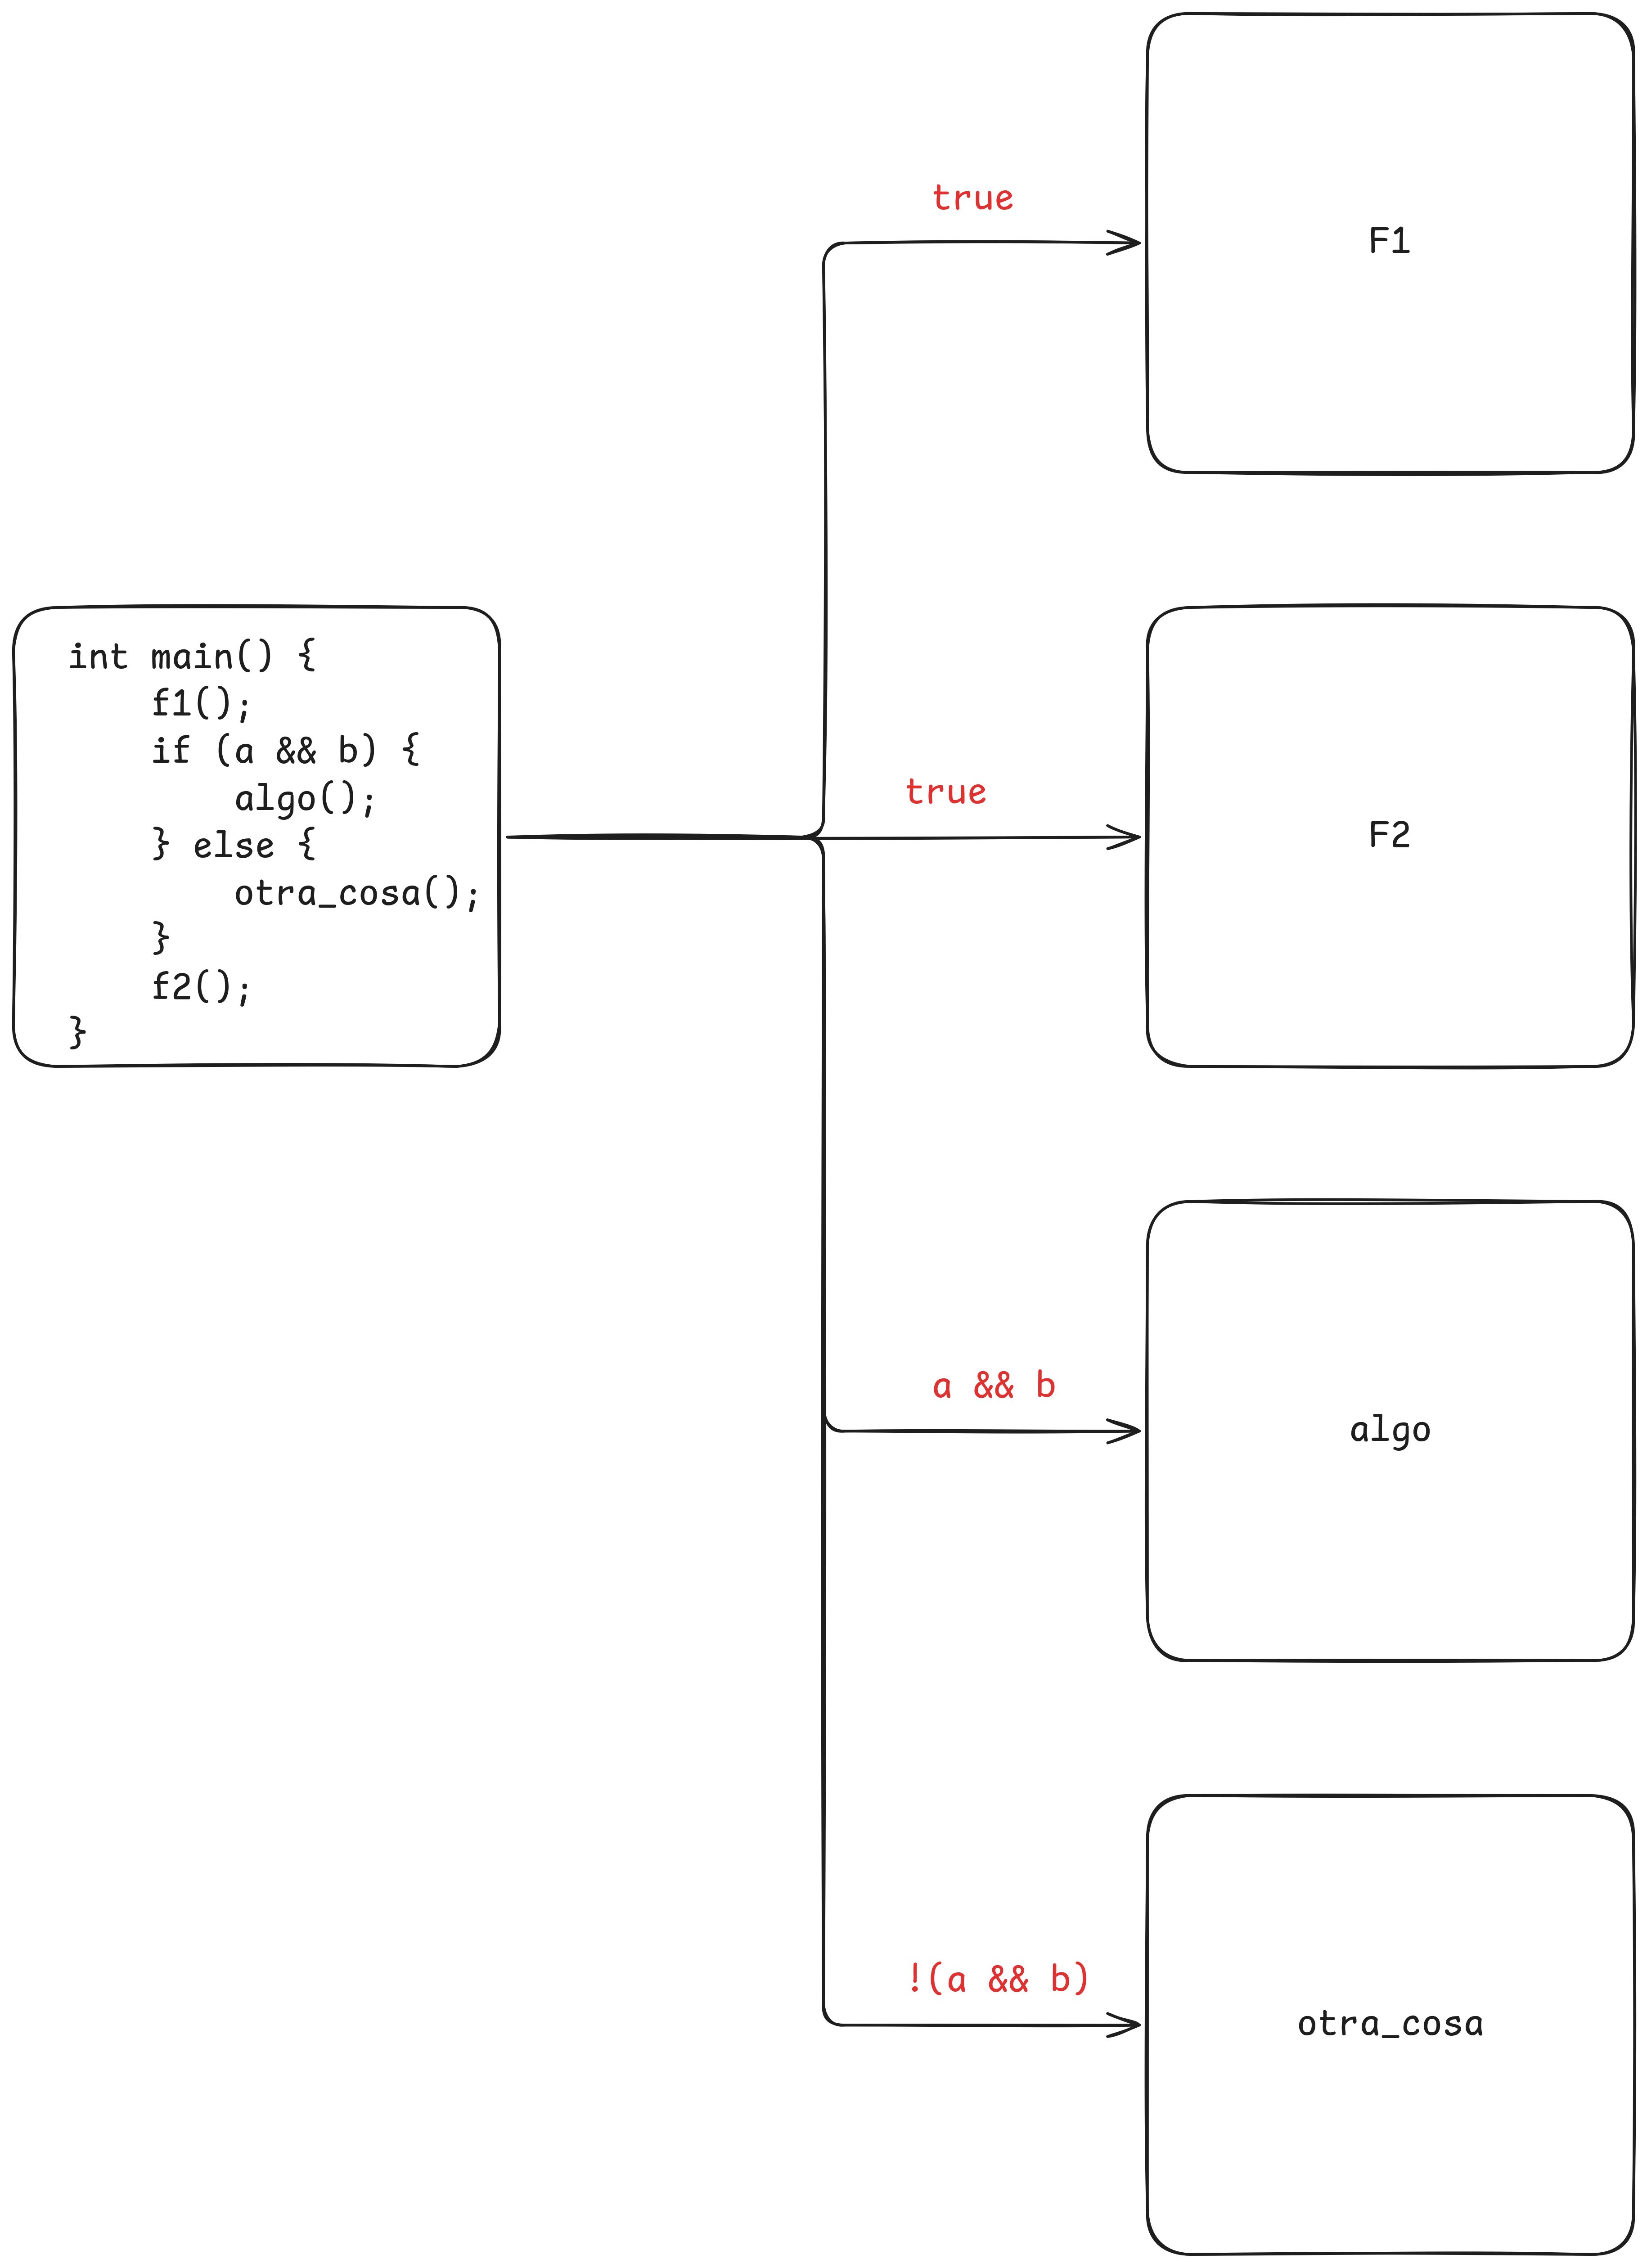
\includegraphics[width=0.6\linewidth]{./images/Ramas_Simple.png}
  \caption{Árbol de ejecución de un programa simple. Nótese como cada función genera su propio bloque y algunas ramas tienen condiciones que deben cumplirse para ser ejecutadas.}
  \label{fig:branch_simple}
\end{figure}

  Éste árbol es justamente lo que programas como AFL++ exploran y es la segunda estrategia que usaron en SQLite para aliviar los bugs \cite{software_should_work_2026}. Su objetivo es variar de forma automática varios inputs del programa, lo que a su vez varía las condicinoes de ejecución de ciertas ramas, reportando solamente las ramas que hacen que el programa falle alguno de los chequeos que el programador defina, lo que a su vez ayuda a descubrir caminos que rara vez son ejecutados normalmente \cite{bohme2020fuzzing}. Hay dos tipos principales de \textit{fuzzing}:
	\begin{itemize}
\item Mutacional: La campaña de fuzzing inicia con varias "semillas". Luego estas semillas son modificadas para generar nuevas entradas al programa.
		\item Generacional: Las entradas son generadas desde 0, si se especifica un formato entonces se generan entradas que cumplan ese formato. Solamente las entradas que más profundo lleguen a explorar el sistema son evolucionadas a la siguiente ronda \cite{bohme2020fuzzing}.
	\end{itemize}

  \subsubsection{LLMs}
	Richar Hipp menciona que recientemente, a pesar de todos los pasos que ha tomado para asegurarse que el código de SQLite es lo más libre de bugs posible, los \textit{Large Language Models} (LLMs) han encontrado formas exóticas de ejecución de código que revelan vulnerabilidades en su código \cite{software_should_work_2026}.

  Por lo tanto los LLMs deben ser considerados, cuanto mínimo, como un linter más que pueden ayudar a revisar el código y proponer mejoras. Curiosamente, este uso no se alinea más a las propiedades innatas de ellos, siendo estocásticos y alucinando de vez en cuando.

	\subsection{DST}
	TigerBeetle, una de las bases de datos transaccionales más nuevas del mercado, y a la vez, es una que utiliza la estrategia de \textit{Deterministic Simulation Testing} (DST) con gran efectividad para encontrar vulnerabilidades dentro de su software \cite{greef-2023}. Esta técnica de pruebas es mucho más compleja que las descritas anteriormente debido a que necesita de dos factores clave:

	\begin{itemize}

		\item Control de la randomización: Muchos programas y aplicaciones tienen una fuente de randomización, puede que sea una dependencia o el mismo sistema operativo. DST simplemente asume que se tiene una única fuente de randomización en todo el programa, que se controla por una semilla y el simulador tiene el poder de cambiar esa semilla. Esto incluye todas las operaciones de I/O como lo es archivos y llamadas de red.
		\item Control del tiempo: Otra fuente enorme de incertidumbre es el tiempo, DST asume que debes ser capaz de controlar el reloj durante la simulación, no tiene que ser literal, Phil Eaton (uno de los investigadores de TigerBeetle) explica que esto se traduce a que cada vez que querramos obtener el tiempo dentro de nuestra aplicación, en su lugar deberíamos interactuar con una interfaz cuya implementación podamos cambiar luego dentro del simulador \cite{eaton-2024}.
	\end{itemize}

	Una clara desventaja de esta metodología de pruebas es que el core de nuestro sistema no puede tener múltiples hilos o por lo menos, debemos soportar una forma de correr múltiples instancias o nodos dentro de un mismo proceso, esto se debe a que es el sistema operativo el encargado de manejar la calendarización de procesos e hilos que los programas crean, por lo tanto, manejar esta calendarización de forma determinista implicaría escribir un sistema operativo personalizado para la aplicación \cite{eaton-2024}.

	Otro punto a tomar en cuenta cuando se desarrollan sistemas para aplicarles DST son lo que Phil llama aristas. Tarde o temprano la aplicación deberá interactuar con partes que no son deterministas, justamente estas partes son las que estamos empaquetando en una interfaz y simulando dentro del DST. Estas son las aristas de la aplicación. Mientras más aristas tengamos menos código real estaremos probando y por lo tanto, las recompensas de aplicar DST disminuyen, por lo tanto es importante maximizar la cantidad de código que podemos revisar y que esté dentro de lo que el simulador prueba y el código final que compilaremos a producción \cite{eaton-2024}.

	Por último, Will Wilson recalca que lo más difícil de construir un DST no es el DST en sí mismo, es verificar que está funcionando correctamente, es decir, que efectivamente está explorando casos interesantes dentro de el código encontrando bugs. Según él, es muy sencillo construir un simulador que finge estar trabajando cuando en realidad no está explorando mucho del espacio de posibles estados (ver \ref{fig:branch_simple}) del sistema. Además, menciona que desafortunadamente y a diferencia de \textit{fuzzing} no se puede usar el \textit{branch coverage} como guía, y generalmente es una métrica muy mala para la clase de sistemas que querrías probar con DST \cite{eaton-2024}.
